\documentclass[12pt,a4paper]{report}

% ══════════════════════════════════════════════════════════════════════════
% PACKAGES
% ══════════════════════════════════════════════════════════════════════════
\usepackage[utf8]{inputenc}
\usepackage[T1]{fontenc}
\usepackage[french]{babel}
\usepackage[margin=2.5cm]{geometry}
\usepackage{mathptmx}
\usepackage{setspace}
\usepackage{titlesec}
\usepackage{graphicx}
\usepackage{caption}
\usepackage{xcolor}
\definecolor{emsigreen}{RGB}{88,150,60}
\usepackage{fancyhdr}
\usepackage{hyperref}
\usepackage{indentfirst}
\usepackage{tocloft}
\usepackage{array}
\usepackage{booktabs}
\usepackage{float}
\usepackage{needspace}
\usepackage{placeins}
\usepackage{listings}
\lstset{
    basicstyle=\ttfamily\footnotesize,
    keywordstyle=\color{emsigreen}\bfseries,
    commentstyle=\color{black!50}\itshape,
    stringstyle=\color{black!70},
    numbers=left,
    numberstyle=\tiny\color{black!40},
    frame=single,
    breaklines=true,
    tabsize=4,
    showstringspaces=false,
    captionpos=b
}
\usepackage{tikz}
\usepackage{pgfgantt}
\usetikzlibrary{shapes.geometric, arrows.meta, positioning, fit, backgrounds}

\onehalfspacing

\titleformat{\section}{\normalfont\fontsize{14}{16}\bfseries}{\thesection}{1em}{}
\titleformat{\subsection}{\normalfont\fontsize{13}{15}\bfseries}{\thesubsection}{1em}{}
\titleformat{\subsubsection}{\normalfont\fontsize{12}{14}\bfseries}{\thesubsubsection}{1em}{}

\captionsetup{font={it,footnotesize},labelfont={it,footnotesize}}

\pagestyle{fancy}
\fancyhf{}
\renewcommand{\headrulewidth}{0.4pt}
\renewcommand{\footrulewidth}{0.4pt}
\fancyfoot[L]{EL FELLAH Adil}
\fancyfoot[R]{Page \thepage}
\fancyhead[L]{\nouppercase{\leftmark}}

\hypersetup{
    colorlinks=true,
    linkcolor=black,
    citecolor=black,
    urlcolor=blue,
    pdftitle={Développement d'une plateforme d'e-services hôteliers},
    pdfauthor={EL FELLAH Adil}
}

\begin{document}

% ─────────────────────────────────────────────────────────────────────────
% PAGE DE GARDE
% ─────────────────────────────────────────────────────────────────────────
\begin{titlepage}
    \thispagestyle{empty}

    \vspace{0.5cm}

    \noindent
    \colorbox{emsigreen}{
        \begin{minipage}{\textwidth}
            \raggedleft
            \vspace{4pt}
            % \includegraphics[width=3.5cm]{logo-emsi.png} % Logo EMSI à ajouter sur Overleaf
            \color{white}\textbf{\Large ÉCOLE MAROCAINE DES SCIENCES DE L'INGÉNIEUR}\\[2pt]
            {\small\color{white} Membre de HONORIS UNITED UNIVERSITIES}
            \vspace{4pt}
        \end{minipage}
    }

    \vspace{2cm}

    \begin{flushright}
        \colorbox{emsigreen}{
            \begin{minipage}{7cm}
                \centering
                \vspace{4pt}
                \color{white}{\huge \textbf{PROJET DE FIN D'ANNÉE}}\\[4pt]
                \color{white}{\Large 2025-2026}
                \vspace{4pt}
            \end{minipage}
        }
    \end{flushright}

    \vspace{1.5cm}

    \noindent\textbf{\Large THÈME}\dotfill

    \vspace{0.5cm}

    \noindent
    \begin{minipage}{0.95\textwidth}
        \centering
        {\Large \textbf{Conception et développement d'une plateforme
        d'e-services hôteliers : Réservation, Room Service et
        Réclamations}}
    \end{minipage}

    \vspace{1.5cm}

    \noindent{\LARGE \textbf{Ingénierie Informatique et Réseaux}}\\[2pt]
    \noindent{\color{emsigreen}\rule{0.6\textwidth}{2pt}}

    \vspace{1.5cm}

    \noindent{\color{emsigreen}\rule{0.06cm}{1cm}}\hspace{0.3cm}
    \begin{minipage}{0.8\textwidth}
        \textbf{Réalisé par :}\\
        EL FELLAH Adil
    \end{minipage}

    \vspace{0.5cm}

    \noindent{\color{emsigreen}\rule{0.06cm}{1cm}}\hspace{0.3cm}
    \begin{minipage}{0.8\textwidth}
        \textbf{Encadré par :}\\
        M./Mme XXXXXXX (EMSI)
    \end{minipage}

    \vspace{0.5cm}

    \noindent{\color{emsigreen}\rule{0.06cm}{1cm}}\hspace{0.3cm}
    \begin{minipage}{0.8\textwidth}
        \textbf{Soutenu le :} XX/XX/2026
    \end{minipage}

    \vfill

\end{titlepage}

% ─────────────────────────────────────────────────────────────────────────
% NUMÉROTATION ROMAINE
% ─────────────────────────────────────────────────────────────────────────
\pagenumbering{roman}
\setcounter{page}{2}

\chapter*{Dédicace}
\addcontentsline{toc}{chapter}{Dédicace}

À mes chers parents, source inépuisable de patience, d'encouragement et
d'amour, qui n'ont jamais cessé de croire en mes capacités et qui ont
consenti tant de sacrifices pour assurer mon éducation dans les meilleures
conditions. Aucune dédicace ne saurait exprimer la profondeur de ma
gratitude envers vous.

À mes frères et sœurs, pour leur soutien moral constant et leurs
encouragements tout au long de mon parcours académique.

À mes professeurs de l'École Marocaine des Sciences de l'Ingénieur, qui
ont su transmettre avec rigueur et passion les connaissances nécessaires à
la réalisation de ce projet, et qui ont contribué, chacun à sa manière, à
forger l'ingénieur que je m'efforce de devenir.

À mes amis et camarades de promotion, pour les moments de partage,
d'entraide et de motivation mutuelle qui ont accompagné ces années
d'études.

À toute personne ayant, de près ou de loin, contribué à l'aboutissement de
ce travail, je dédie ce modeste rapport en signe de reconnaissance et de
profond respect.

\clearpage

\chapter*{Remerciements}
\addcontentsline{toc}{chapter}{Remerciements}

Au terme de ce projet de fin d'année, je tiens à exprimer ma profonde
gratitude envers toutes les personnes qui ont contribué, de près ou de
loin, à sa réalisation.

Je remercie tout particulièrement mon encadrant pédagogique, pour la
qualité de son encadrement, la pertinence de ses conseils et sa
disponibilité constante tout au long de ce projet. Ses orientations
avisées et son exigence intellectuelle m'ont permis de mener ce travail à
son terme dans les meilleures conditions.

Mes remerciements s'adressent également à l'ensemble du corps enseignant
du département Ingénierie Informatique et Réseaux de l'École Marocaine des
Sciences de l'Ingénieur, pour la qualité de la formation dispensée tout au
long de ce cursus et pour les compétences techniques et méthodologiques
qu'ils ont su me transmettre.

Je souhaite également remercier les membres du jury qui me font l'honneur
d'évaluer ce travail, pour le temps qu'ils consacrent à sa lecture et à
son évaluation, ainsi que pour leurs remarques constructives qui
contribueront sans nul doute à son amélioration.

Enfin, mes remerciements vont à toute personne ayant, par ses conseils,
ses remarques ou son soutien, contribué à l'enrichissement de ce travail
et à son bon déroulement.

\clearpage

\chapter*{Résumé}
\addcontentsline{toc}{chapter}{Résumé}

Le secteur hôtelier connaît aujourd'hui une transformation numérique
profonde, dans laquelle la qualité des services digitaux proposés aux
clients constitue un facteur de différenciation majeur. C'est dans ce
contexte que s'inscrit ce projet de fin d'année, qui porte sur la
conception et le développement d'une plateforme web d'e-services destinée
à un établissement hôtelier, l'hôtel Rambla Marrakech.

La problématique traitée consiste à remplacer les échanges manuels
traditionnellement établis entre le client et le personnel de
l'établissement (réservation téléphonique, commande orale au restaurant,
signalement verbal d'un incident technique) par une plateforme numérique
centralisée, capable de servir simultanément trois profils d'utilisateurs
aux besoins distincts.

La plateforme développée repose sur le framework Laravel, dans sa version
12, et propose trois espaces utilisateurs distincts : un espace client, un
espace serveur/restaurant et un espace d'administration et de gestion
technique. Elle prend en charge la réservation de chambres et de services
hôteliers avec vérification de disponibilité en temps réel et calendrier
interactif, la gestion complète du room service depuis la passation de la
commande jusqu'à sa livraison, ainsi que le traitement des réclamations
techniques avec priorisation automatique des incidents jugés critiques.

Le projet a été conduit selon la méthode agile Scrum, organisée en cinq
sprints successifs, chacun ayant donné lieu à un incrément fonctionnel
testable. Une attention particulière a été portée à la sécurisation des
accès par un système de contrôle des rôles, ainsi qu'à la fiabilité des
règles métier critiques, en particulier la prévention rigoureuse des
conflits de réservation sur une même chambre. Les tests réalisés ont
permis de valider le bon fonctionnement de l'ensemble des modules
développés.

\vspace{0.5cm}
\noindent\textbf{Mots-clés :} hôtellerie, plateforme web, Laravel, réservation,
e-services, gestion des rôles, méthode Scrum.

\clearpage

\chapter*{Abstract}
\addcontentsline{toc}{chapter}{Abstract}

The hospitality industry is currently undergoing a profound digital
transformation, in which the quality of digital services offered to guests
has become a major differentiating factor. It is within this context that
this final-year project takes place, focusing on the design and
development of a hotel e-services web platform for the Rambla Marrakech
hotel.

The problem addressed consists in replacing the traditionally manual
exchanges between guests and hotel staff -- phone bookings, verbal
restaurant orders, and word-of-mouth reporting of technical issues -- with
a single centralized digital platform capable of simultaneously serving
three distinct user profiles.

The platform is built on the Laravel framework, version 12, and provides
three distinct user spaces: a guest space, a waiter/restaurant space, and
an administration and technical management space. It supports room and
service bookings with real-time availability checking and an interactive
calendar, complete room-service order management from placement through
delivery, and technical complaint handling with automatic priority
assignment for critical issues.

The project was carried out using the Scrum agile methodology, organized
into five successive sprints, each delivering a testable functional
increment. Particular attention was paid to securing access through a
role-based control system, as well as to the reliability of critical
business rules, especially the rigorous prevention of booking conflicts on
a given room. The tests carried out confirmed the correct functioning of
all developed modules.

\vspace{0.5cm}
\noindent\textbf{Keywords:} hospitality, web platform, Laravel, booking,
e-services, role management, Scrum method.

\clearpage

\chapter*{Liste des abréviations}
\addcontentsline{toc}{chapter}{Liste des abréviations}

\begin{description}
    \item[API :] Application Programming Interface
    \item[BDD :] Base de données
    \item[CRUD :] Create, Read, Update, Delete
    \item[EMSI :] École Marocaine des Sciences de l'Ingénieur
    \item[HTTP :] HyperText Transfer Protocol
    \item[MVC :] Modèle-Vue-Contrôleur
    \item[OAuth :] Open Authorization
    \item[ORM :] Object-Relational Mapping
    \item[PFA :] Projet de Fin d'Année
    \item[SGBD :] Système de Gestion de Base de Données
    \item[SQL :] Structured Query Language
    \item[UML :] Unified Modeling Language
\end{description}

\clearpage

\listoffigures
\addcontentsline{toc}{chapter}{Liste des figures}
\clearpage

\listoftables
\addcontentsline{toc}{chapter}{Liste des tableaux}
\clearpage

\tableofcontents
\clearpage

% ─────────────────────────────────────────────────────────────────────────
% NUMÉROTATION ARABE
% ─────────────────────────────────────────────────────────────────────────
\pagenumbering{arabic}
\setcounter{page}{1}

\chapter*{Introduction générale}
\addcontentsline{toc}{chapter}{Introduction générale}

Le secteur hôtelier connaît une transformation numérique profonde, dans
laquelle la disponibilité de services numériques constitue un facteur
différenciateur majeur pour l'expérience du client. Dans ce contexte,
l'hôtel Rambla Marrakech a servi de cadre à un projet visant à
dématérialiser les principaux échanges entre le client et le personnel de
l'établissement. La plateforme développée centralise la réservation de
chambres et de prestations, la commande de room service, ainsi que la
remontée et le traitement des réclamations techniques.

Ce rapport est organisé en cinq chapitres :

\begin{itemize}
    \item Le premier chapitre présente le contexte général du projet, la
    problématique, les objectifs, le cahier des charges ainsi que la
    méthodologie de gestion de projet adoptée.
    \item Le deuxième chapitre détaille la conception et le développement
    de la plateforme e-services hôteliers.
    \item Le troisième chapitre présente l'étude technique : langages,
    frameworks, outils de développement et architecture retenus.
    \item Le quatrième chapitre présente les tests réalisés, les résultats
    obtenus ainsi que les perspectives d'amélioration.
    \item Le cinquième chapitre présente la mise en \oe uvre du projet :
    structure générale et principales interfaces de l'application.
\end{itemize}

\clearpage

% ═════════════════════════════════════════════════════════════════════════
% CHAPITRE 1
% ═════════════════════════════════════════════════════════════════════════
\chapter{Contexte général et cadre du projet}

\section{Introduction}

Ce premier chapitre présente le cadre général dans lequel s'inscrit le
projet. Il expose le contexte, la problématique identifiée, les objectifs
poursuivis, le cahier des charges fonctionnel, la méthodologie de gestion
de projet ainsi que les choix technologiques qui ont guidé la conception
et le développement.

\section{Présentation du contexte}

L'hôtel Rambla Marrakech est un établissement hôtelier proposant des
chambres de différentes catégories (simple, double, suite) ainsi que des
prestations annexes telles que le spa, la navette aéroport ou la location
de vélo. Comme dans la majorité des établissements de taille comparable,
la gestion quotidienne des demandes des clients repose historiquement sur
des échanges directs entre le client et le personnel : appel téléphonique
depuis la chambre vers la réception ou le restaurant, déplacement
physique, ou transmission orale d'une information au personnel technique
en cas de panne.

\subsection{Étude de l'existant}

Cette organisation manuelle présente plusieurs limites. Elle ne permet pas
de conserver un historique structuré des demandes, ce qui complique le
suivi d'une réclamation ou d'une commande dans le temps. Elle repose
fortement sur la disponibilité immédiate du personnel, ce qui peut générer
des délais de prise en charge variables selon les périodes d'affluence.
Elle ne permet pas non plus au client de visualiser, avant sa réservation,
les caractéristiques précises d'une chambre (photographies, équipements,
surface) ni sa disponibilité réelle sur une période donnée, ce qui peut
conduire à des doubles réservations nécessitant une intervention manuelle
de correction.

\subsection{État de l'art}

Le marché des logiciels de gestion hôtelière (\textit{Property Management
System}, ou PMS) propose plusieurs solutions établies, telles qu'Opera
PMS, Cloudbeds ou Mews. Ces plateformes couvrent généralement la gestion
des réservations, la facturation et le suivi de l'occupation des chambres
à destination du personnel de l'hôtel. Toutefois, ces solutions
commerciales restent principalement orientées vers la gestion interne de
l'établissement et proposent rarement une interface dédiée et directement
accessible au client depuis sa propre chambre pour des besoins aussi
variés que la commande de room service ou le signalement d'un incident
technique.

Cette observation a orienté la conception du présent projet vers une
plateforme centrée sur trois usages complémentaires -- client, personnel
de restauration et personnel technique/administratif -- plutôt que vers un
outil de gestion hôtelière généraliste. Ce choix permet de répondre de
façon ciblée aux besoins fonctionnels exprimés par l'établissement,
tout en conservant une architecture suffisamment simple pour rester
maintenable par une équipe de taille réduite.

\subsection{Problématique}

Le projet répond à la problématique suivante : comment remplacer les
échanges manuels entre client et personnel par une plateforme numérique
unique, capable de centraliser les réservations, les commandes de room
service et les réclamations techniques, tout en garantissant que chaque
acteur (client, serveur, personnel technique et administratif) dispose
d'un espace de travail adapté à son rôle, et que les règles métier
critiques -- en particulier l'absence de conflit entre deux réservations
sur une même chambre -- soient appliquées de manière fiable et automatique.

\subsection{Objectifs du projet}

Le projet poursuit les objectifs suivants :
\begin{itemize}
    \item permettre au client de consulter les chambres disponibles avec
    leurs caractéristiques détaillées et de réserver une chambre ou un
    service sur un créneau donné, avec une vérification automatique de
    disponibilité ;
    \item offrir au client la possibilité de commander au room service et
    de suivre la préparation de sa commande ;
    \item offrir au client un moyen simple de signaler un incident
    technique dans sa chambre ;
    \item offrir au personnel de restauration une interface de suivi des
    commandes en cours, de leur réception jusqu'à leur livraison ;
    \item offrir au personnel technique et administratif une interface de
    gestion des réclamations, avec mise en évidence automatique des
    incidents critiques, ainsi qu'une interface de validation des
    réservations ;
    \item garantir l'étanchéité des accès entre les différents rôles
    d'utilisateurs.
\end{itemize}

\section{Cahier des charges}

Le cahier des charges fonctionnel se décline selon les trois espaces
utilisateurs de la plateforme, résumés dans le tableau~\ref{tab:cahier}.

\begin{table}[H]
\centering
\begin{tabular}{p{3cm} p{9cm}}
\toprule
\textbf{Espace} & \textbf{Fonctionnalités principales} \\
\midrule
Client & Consultation des chambres, réservation avec vérification de
disponibilité, annulation, commande de room service, dépôt de
réclamations \\
Serveur / Restaurant & Suivi des commandes en cours, mise à jour du statut
de préparation et de livraison \\
Administration / Technique & Gestion et priorisation des réclamations,
validation ou annulation des réservations en attente \\
\bottomrule
\end{tabular}
\caption{Synthèse du cahier des charges fonctionnel}
\label{tab:cahier}
\end{table}

L'accès à chacun de ces espaces est conditionné par le rôle attribué à
l'utilisateur, ce rôle étant vérifié à chaque requête par un mécanisme de
contrôle d'accès dédié, détaillé au chapitre suivant.

\section{Contraintes du projet}

Le développement de la plateforme a dû répondre à plusieurs contraintes.
Une contrainte de cohérence des données a imposé la mise en place d'une
vérification stricte des chevauchements de dates pour les réservations de
chambres, afin d'éviter qu'une même chambre puisse être réservée
simultanément par deux clients différents. Une contrainte d'ergonomie a
orienté la conception de l'interface vers une identité visuelle cohérente
et une expérience utilisateur fluide sur l'ensemble des espaces. Enfin,
une contrainte de sécurité a imposé une séparation stricte des
permissions entre les différents rôles d'utilisateurs.

\section{Méthodologie de gestion de projet (Scrum)}

\subsection{Présentation du framework Scrum}

La réalisation de la plateforme Rambla Marrakech a suivi le framework
agile \textbf{Scrum}, dont le principe central consiste à découper le
développement en itérations courtes et planifiées appelées
\textit{sprints}. Chaque sprint produit un incrément fonctionnel et
testable, permettant un ajustement continu des priorités en fonction des
retours obtenus.

Les rôles définis dans ce cadre sont les suivants :

\begin{itemize}
    \item \textbf{Product Owner} : responsable de la définition et de la
    priorisation du \textit{backlog} produit, garant de la valeur
    fonctionnelle de chaque livraison.
    \item \textbf{Scrum Master} : facilitateur chargé de lever les
    obstacles et de veiller au respect des cérémonies Scrum (planning,
    revue, rétrospective).
    \item \textbf{Équipe de développement} : réalise les éléments du
    backlog sélectionnés pour chaque sprint.
\end{itemize}

\subsection{Déroulement des sprints}

Le développement a été organisé en cinq sprints successifs, chacun ciblant
un module fonctionnel précis :

\begin{itemize}
    \item \textbf{Sprint 0 (Initialisation)} : mise en place de
    l'environnement Laravel 12, configuration de la base de données,
    scaffolding d'authentification, création des migrations initiales.
    \item \textbf{Sprint 1 (Espace Client -- Réservations)} : développement
    du module de consultation des chambres, du formulaire de réservation
    avec vérification de disponibilité en temps réel et de la politique
    d'annulation à 24 heures.
    \item \textbf{Sprint 2 (Room Service)} : implémentation de la carte de
    menu groupée par catégorie, création des commandes avec calcul
    automatique du total, et suivi des livraisons.
    \item \textbf{Sprint 3 (Réclamations)} : module de dépôt de
    réclamations avec priorisation automatique, espace d'administration
    avec assignation à un technicien.
    \item \textbf{Sprint 4 (Administration et finalisation)} : gestion des
    réservations côté admin, intégration de l'authentification OAuth
    Google, tests fonctionnels et corrections.
\end{itemize}

\subsection{Planification du projet (diagramme de Gantt)}

La Figure~\ref{fig:gantt} présente la planification globale du projet sous
forme de diagramme de Gantt, répartie sur seize semaines.

\begin{figure}[H]
    \centering
    \begin{ganttchart}[
        hgrid,
        vgrid={*{1}{dotted}},
        x unit=0.72cm,
        y unit title=0.6cm,
        y unit chart=0.55cm,
        title/.style={fill=black!80, draw=none},
        title label font=\color{white}\scriptsize\bfseries,
        bar/.style={fill=black!55, rounded corners=1pt},
        bar label font=\scriptsize,
        group/.style={fill=black!25},
        group label font=\scriptsize\bfseries
    ]{1}{16}
        \gantttitle{Semaines}{16} \\
        \gantttitlelist{1,...,16}{1} \\
        \ganttgroup{Analyse \& Conception}{1}{3} \\
        \ganttbar{Étude des besoins}{1}{2} \\
        \ganttbar{Modélisation UML}{2}{3} \\
        \ganttgroup{Sprint 0 -- Initialisation}{3}{4} \\
        \ganttbar{Env. dev. + migrations}{3}{4} \\
        \ganttgroup{Sprint 1 -- Réservations}{4}{7} \\
        \ganttbar{Chambres + photos}{4}{5} \\
        \ganttbar{Module réservation}{5}{7} \\
        \ganttgroup{Sprint 2 -- Room Service}{7}{9} \\
        \ganttbar{Carte de menu + commandes}{7}{9} \\
        \ganttgroup{Sprint 3 -- Réclamations}{9}{11} \\
        \ganttbar{Dépôt + priorisation}{9}{11} \\
        \ganttgroup{Sprint 4 -- Administration}{11}{13} \\
        \ganttbar{Espace admin réservations}{11}{12} \\
        \ganttbar{OAuth Google}{12}{13} \\
        \ganttgroup{Tests \& Corrections}{13}{15} \\
        \ganttbar{Tests fonctionnels}{13}{14} \\
        \ganttbar{Corrections et polish}{14}{15} \\
        \ganttgroup{Rédaction du rapport}{1}{16} \\
        \ganttbar{Rédaction continue}{1}{16}
    \end{ganttchart}
    \caption{Diagramme de Gantt du projet Rambla Marrakech}
    \label{fig:gantt}
\end{figure}

\section{Méthodologie et technologies adoptées}

Les technologies retenues pour la partie applicative sont les suivantes.
\textbf{Laravel 12} a été choisi comme framework PHP principal en raison
de son architecture MVC mature, de son ORM Eloquent qui simplifie la
gestion des relations polymorphiques, et de son écosystème riche (Breeze
pour l'authentification, Socialite pour OAuth, Tinker pour les tests en
console). \textbf{MySQL} est utilisé comme système de gestion de base de
données. \textbf{Tailwind CSS} assure la cohérence visuelle via un
système de design basé sur des tokens de couleurs personnalisés.
\textbf{Flatpickr} fournit les sélecteurs de dates et d'heures avec
désactivation dynamique des plages déjà réservées. \textbf{Laravel
Socialite} assure l'authentification via OAuth 2.0 avec Google.

\section{Conclusion}

Ce chapitre a permis de situer le projet dans son contexte, d'en formuler
la problématique et les objectifs, et de présenter le cahier des charges,
les contraintes ainsi que la méthodologie Scrum et les choix technologiques
retenus. Le chapitre suivant détaille la conception et le développement de
la plateforme e-services.

% ═════════════════════════════════════════════════════════════════════════
% CHAPITRE 2
% ═════════════════════════════════════════════════════════════════════════
\chapter{Conception et développement de la plateforme e-services}

\section{Introduction}

Ce chapitre présente la conception et le développement de la plateforme
web d'e-services hôteliers. Il détaille l'analyse fonctionnelle, le modèle
de données, les choix technologiques retenus, le fonctionnement de chacun
des trois espaces utilisateurs, ainsi que le mécanisme de gestion des
rôles et de sécurité mis en place.

\section{Analyse et conception}

La conception de la plateforme s'est appuyée sur une identification des
acteurs du système et de leurs interactions, ainsi que sur la définition
d'un modèle de données relationnel couvrant l'ensemble des besoins
fonctionnels exprimés dans le cahier des charges.

\subsection{Diagramme de cas d'utilisation}

Trois acteurs interagissent avec le système. Le client peut consulter les
chambres disponibles, créer une réservation, l'annuler sous certaines
conditions, passer une commande de room service et déposer une
réclamation. Le serveur peut consulter les commandes en cours et modifier
leur statut de préparation. Le personnel d'administration et technique
peut consulter les réclamations, les assigner et les résoudre, ainsi que
confirmer ou annuler les réservations en attente. La Figure~\ref{fig:usecase}
présente le diagramme de cas d'utilisation global de la plateforme.

\begin{figure}[H]
    \centering
    \begin{tikzpicture}[
        actoricon/.style={circle, fill=black!15, minimum size=0.6cm},
        actorlabel/.style={font=\small\bfseries, text centered},
        usecase/.style={
            ellipse, draw, fill=black!8,
            text centered, font=\small,
            minimum width=3.4cm, minimum height=0.65cm,
            inner sep=1pt
        },
        system/.style={
            rectangle, draw, thick,
            inner sep=10pt, rounded corners=4pt
        }
    ]
        \node[actoricon] (clienticon) at (-5.5, 3.05) {};
        \node[actorlabel, below=2pt of clienticon] (client) {Client};

        \node[actoricon] (serveuricon) at (-5.5, 0.25) {};
        \node[actorlabel, below=2pt of serveuricon] (serveur) {Serveur};

        \node[actoricon] (adminicon) at (-5.5, -2.55) {};
        \node[actorlabel, below=2pt of adminicon] (admin) {Admin / Tech.};

        \node[usecase] (uc1) at (0,  4.4) {Consulter les chambres};
        \node[usecase] (uc2) at (0,  3.2) {Réserver (chambre/service)};
        \node[usecase] (uc3) at (0,  2.0) {Annuler une réservation};
        \node[usecase] (uc4) at (0,  0.8) {Passer une commande};
        \node[usecase] (uc5) at (0, -0.4) {Déposer une réclamation};
        \node[usecase] (uc6) at (0, -1.6) {Gérer les commandes};
        \node[usecase] (uc7) at (0, -2.8) {Gérer les réservations};
        \node[usecase] (uc8) at (0, -4.0) {Traiter les réclamations};
        \node[usecase] (uc9) at (0, -5.2) {Tableau de bord};

        \begin{scope}[on background layer]
            \node[system, fit=(uc1)(uc2)(uc3)(uc4)(uc5)(uc6)(uc7)(uc8)(uc9),
                  label={[font=\small\bfseries]above:Plateforme Rambla Marrakech}
            ] (sys) {};
        \end{scope}

        \draw (client) -- (uc1);
        \draw (client) -- (uc2);
        \draw (client) -- (uc3);
        \draw (client) -- (uc4);
        \draw (client) -- (uc5);
        \draw (serveur) -- (uc6);
        \draw (admin) -- (uc7);
        \draw (admin) -- (uc8);
        \draw (admin) -- (uc9);
    \end{tikzpicture}
    \caption{Diagramme de cas d'utilisation de la plateforme Rambla Marrakech}
    \label{fig:usecase}
\end{figure}

\subsection{Modèle de données (diagramme de classes)}

Le modèle de données s'articule autour de neuf tables principales,
résumées dans le tableau~\ref{tab:tables}.

\begin{table}[H]
\centering
\begin{tabular}{p{3cm} p{9cm}}
\toprule
\textbf{Table} & \textbf{Rôle} \\
\midrule
users & Utilisateurs, rôle (client, serveur, technicien, administrateur),
chambre associée \\
rooms & Chambres : numéro, étage, type, statut, prix, surface, capacité,
type de lit, équipements \\
room\_photos & Photographies associées à chaque chambre \\
services & Prestations proposées par l'hôtel (spa, navette, etc.) \\
reservations & Réservations, relation polymorphe vers une chambre ou un
service, statut et créneau \\
menu\_items & Articles du menu du restaurant, organisés par catégorie \\
orders & Commandes de room service, statut de préparation, montant total \\
order\_items & Articles composant chaque commande, quantité \\
complaints & Réclamations techniques, type, priorité, statut \\
\bottomrule
\end{tabular}
\caption{Principales tables du modèle de données}
\label{tab:tables}
\end{table}

La table \texttt{reservations} constitue une relation polymorphe : elle
peut porter indifféremment sur une chambre ou sur un service, ce qui évite
la duplication de la logique de réservation entre ces deux types
d'éléments réservables. Chaque réservation porte un statut parmi
\emph{en\_attente}, \emph{confirmee}, \emph{annulee} et \emph{terminee}.
La Figure~\ref{fig:classes} présente le diagramme de classes simplifié
correspondant.

\begin{figure}[H]
    \centering
    \begin{tikzpicture}[
        class/.style={
            rectangle, draw, thick, fill=black!6,
            font=\scriptsize, align=left,
            minimum width=3.0cm
        },
        header/.style={
            rectangle, draw, thick, fill=black!30,
            text=white, font=\scriptsize\bfseries,
            minimum width=3.0cm, minimum height=0.55cm,
            text centered
        },
        rel/.style={->, >=Stealth, thick},
        comp/.style={->, >=diamond, thick},
        poly/.style={->, >=open diamond, thick, dashed}
    ]
        \node[header] (uh) at (0, 8.5) {users};
        \node[class, anchor=north] (u) at (0, 8.18)
            {id, name, email, role\\room\_id (FK)};

        \node[header] (rh) at (4.8, 8.5) {rooms};
        \node[class, anchor=north] (r) at (4.8, 8.18)
            {id, number, floor, type\\status, price\_per\_night\\wifi\_vlan, amenities (JSON)};

        \node[header] (ph) at (4.8, 5.8) {room\_photos};
        \node[class, anchor=north] (p) at (4.8, 5.48)
            {id, room\_id (FK)\\url, position};

        \node[header] (resh) at (0, 5.8) {reservations};
        \node[class, anchor=north] (res) at (0, 5.48)
            {id, user\_id (FK)\\reservable\_type\\reservable\_id\\start/end\_datetime\\status, total\_price};

        \node[header] (svh) at (9.2, 8.5) {services};
        \node[class, anchor=north] (sv) at (9.2, 8.18)
            {id, name, price\\is\_active};

        \node[header] (oh) at (0, 2.4) {orders};
        \node[class, anchor=north] (o) at (0, 2.08)
            {id, user\_id (FK)\\room\_id (FK), served\_by\\status, total\_amount};

        \node[header] (oih) at (4.8, 2.4) {order\_items};
        \node[class, anchor=north] (oi) at (4.8, 2.08)
            {id, order\_id (FK)\\menu\_item\_id (FK)\\quantity, unit\_price};

        \node[header] (mih) at (9.2, 2.4) {menu\_items};
        \node[class, anchor=north] (mi) at (9.2, 2.08)
            {id, name, category\\price, is\_available};

        \node[header] (ch) at (0, -0.5) {complaints};
        \node[class, anchor=north] (c) at (0, -0.82)
            {id, user\_id (FK)\\room\_id (FK), assigned\_to\\type, priority, status\\resolved\_at};

        \draw[rel] (u.east) -- node[above,font=\scriptsize]{occupe} (r.west);
        \draw[comp] (r.south) -- node[right,font=\scriptsize]{1..n} (p.north);
        \draw[rel] (res.north) -- node[right,font=\scriptsize]{n..1} (u.south);
        \draw[poly] (res.east) -- node[above,font=\scriptsize]{réservable} (r.south west);
        \draw[poly] (res.north east) to[bend left=15] node[above,font=\scriptsize]{réservable} (sv.south west);
        \draw[rel] (o.north) to[bend right=10] node[left,font=\scriptsize]{n..1} (u.south);
        \draw[comp] (o.east) -- node[above,font=\scriptsize]{1..n} (oi.west);
        \draw[rel] (oi.east) -- node[above,font=\scriptsize]{n..1} (mi.west);
        \draw[rel] (c.north) to[bend left=10] node[left,font=\scriptsize]{user\_id / assigned\_to}(u.south);
    \end{tikzpicture}
    \caption{Diagramme de classes simplifié de la plateforme Rambla Marrakech}
    \label{fig:classes}
\end{figure}

\section{Choix technologiques}

L'architecture logicielle de la plateforme repose sur le patron
Modèle-Vue-Contrôleur (MVC) implémenté par le framework Laravel 12. Ce
choix s'explique par plusieurs raisons concrètes : la gestion native des
migrations de base de données garantit une évolution contrôlée du schéma ;
l'ORM Eloquent offre une abstraction cohérente des relations entre
entités, y compris les relations polymorphiques nécessaires au module de
réservation ; le moteur de templates Blade simplifie la séparation entre
logique métier et présentation ; enfin, le système de middleware permet
d'appliquer les règles de contrôle d'accès de manière centralisée et
réutilisable.

Tailwind CSS est utilisé pour la construction de l'interface utilisateur.
Le projet définit un système de design propre, basé sur des tokens de
couleurs nommés et des classes utilitaires personnalisées. Laravel
Socialite assure l'intégration OAuth 2.0 avec Google, permettant aux
clients de s'authentifier sans créer de mot de passe local.

\section{Les trois espaces de l'application}

\subsection{Espace Client}

L'espace client regroupe l'ensemble des fonctionnalités accessibles à un
utilisateur authentifié avec le rôle \texttt{client}. Le module de
réservation permet au client de consulter les chambres disponibles avec
leurs caractéristiques et photographies, puis de sélectionner un créneau à
l'aide d'un calendrier interactif. Le client conserve la possibilité
d'annuler une réservation tant que la date d'arrivée demeure éloignée de
plus de vingt-quatre heures. Le module de room service présente le menu
du restaurant organisé par catégorie et permet de composer une commande
dont le montant total est calculé automatiquement. Le module de
réclamation propose une liste de types d'incidents prédéfinis, certains
déclenchant automatiquement une priorité urgente, comme le montre le
Tableau~\ref{tab:priorite}.

\begin{table}[H]
\centering
\begin{tabular}{p{5cm} p{5cm}}
\toprule
\textbf{Type de réclamation} & \textbf{Priorité par défaut} \\
\midrule
Climatisation & Urgente \\
Eau chaude & Urgente \\
Électricité & Urgente \\
Télévision, Wi-Fi, plomberie, autre & Moyenne \\
\bottomrule
\end{tabular}
\caption{Règle de priorisation automatique des réclamations}
\label{tab:priorite}
\end{table}

\subsection{Espace Serveur / Restaurant}

L'espace serveur affiche l'ensemble des commandes de room service non
encore livrées, triées par ordre chronologique. Pour chaque commande, le
personnel de restauration dispose du détail des articles, de la chambre
concernée et du montant total, et peut faire progresser le statut de la
commande selon une séquence strictement ordonnée, présentée dans le
Tableau~\ref{tab:statuts}.

\begin{table}[H]
\centering
\begin{tabular}{p{2cm} p{9cm}}
\toprule
\textbf{Statut} & \textbf{Description} \\
\midrule
Reçue & Commande transmise par le client, en attente de prise en charge \\
En préparation & Commande en cours de préparation par le restaurant \\
En livraison & Commande en route vers la chambre du client \\
Livrée & Commande remise au client, retirée de la liste active \\
\bottomrule
\end{tabular}
\caption{Cycle de vie d'une commande de room service}
\label{tab:statuts}
\end{table}

\subsection{Espace Administration / Technique}

L'espace administration et technique regroupe la gestion des réclamations
et des réservations. Le tableau de bord affiche en évidence le nombre de
réclamations urgentes non résolues. La liste des réclamations met en avant
les incidents prioritaires et permet leur assignation à un technicien
ainsi que leur clôture. La gestion des réservations permet de confirmer ou
d'annuler les réservations en attente.

\section{Sécurité et gestion des rôles}

L'accès aux différents espaces de l'application est contrôlé par un
middleware dédié, appliqué à chaque groupe de routes. Ce middleware
compare le rôle de l'utilisateur authentifié à la liste des rôles
autorisés pour la route demandée, et retourne une erreur d'accès refusé
dans le cas contraire.

\section{Conclusion}

Ce chapitre a présenté la conception du modèle de données ainsi que le
fonctionnement détaillé des trois espaces de la plateforme, en mettant en
évidence les mécanismes de disponibilité en temps réel, de priorisation
des réclamations et de contrôle d'accès par rôle. Le chapitre suivant
présente l'étude technique du projet : langages, frameworks, outils et
architecture retenus.


% ═════════════════════════════════════════════════════════════════════════
% CHAPITRE 3 — ÉTUDE TECHNIQUE
% ═════════════════════════════════════════════════════════════════════════
\chapter{Étude technique}

\section{Introduction}

Dans ce chapitre, nous présentons l'environnement matériel et logiciel du
projet, en détaillant les langages de programmation, les frameworks, les
outils de développement ainsi que l'architecture technique retenue pour la
réalisation de la plateforme.

\section{Environnement matériel et logiciel}

Le développement a été réalisé sur un poste de travail équipé du système
d'exploitation Windows, à l'aide d'un environnement de serveur local
(Laragon) fournissant PHP, MySQL et un serveur web intégré. L'exécution de
l'application en développement s'effectue via le serveur de développement
intégré à Laravel (\texttt{php artisan serve}), couplé au serveur de
développement Vite pour la compilation à chaud des ressources CSS et
JavaScript.

\section{Langages de programmation}

\subsection{PHP}

PHP constitue le langage principal du projet, utilisé côté serveur pour
l'ensemble de la logique métier, des contrôleurs et des modèles de
l'application. Il s'agit d'un langage de script open source largement
répandu dans le développement web, sur lequel repose le framework Laravel.

\subsection{JavaScript}

JavaScript est utilisé côté client pour les comportements interactifs ne
nécessitant pas de rechargement de page : gestion du calendrier de
réservation, mise à jour dynamique de la prévisualisation d'une chambre,
vérification de disponibilité en temps réel via des requêtes
asynchrones, ainsi que les interactions de la galerie photographique.

\subsection{SQL}

Le langage SQL est utilisé indirectement au travers de l'ORM Eloquent de
Laravel, qui génère les requêtes nécessaires à la manipulation de la base
de données MySQL (sélection, insertion, mise à jour et suppression des
enregistrements, jointures entre tables).

\subsection{Blade}

Blade est le moteur de gabarits (\textit{templates}) natif de Laravel,
utilisé pour la génération dynamique des pages HTML de l'application. Il
permet l'inclusion de composants réutilisables, l'héritage de mise en page
et l'intégration de structures de contrôle (conditions, boucles)
directement dans les vues.

\section{Frameworks et bibliothèques}

\subsection{Laravel}

Laravel, dans sa version 12, constitue le framework principal de
l'application côté serveur. Il fournit une architecture
Modèle-Vue-Contrôleur complète, un système de migrations pour la gestion
versionnée du schéma de base de données, un ORM (Eloquent) pour la
manipulation orientée objet des données, ainsi qu'un système
d'authentification (Breeze) et d'intégration OAuth (Socialite).

\subsection{Tailwind CSS}

Tailwind CSS est un framework CSS de type \textit{utility-first}, employé
pour la construction de l'ensemble des interfaces de l'application. Il
permet de définir un système de design cohérent, fondé sur des classes
utilitaires composables et des tokens de couleurs personnalisés.

\subsection{Alpine.js}

Alpine.js est une bibliothèque JavaScript légère, utilisée pour la gestion
d'états d'interface simples (menus déroulants, galeries d'images,
affichage conditionnel) sans nécessiter de framework front-end complet.

\subsection{Flatpickr}

Flatpickr est une bibliothèque JavaScript spécialisée dans la sélection de
dates et d'heures, intégrée au formulaire de réservation pour remplacer
les champs natifs du navigateur par un calendrier visuel permettant de
désactiver dynamiquement les dates déjà réservées.

\section{Outils de développement}

\subsection{Gestion de versions}

Le suivi des modifications du code source est assuré par le système de
contrôle de version Git, couplé à une plateforme d'hébergement distante
(GitHub) permettant la sauvegarde du dépôt et le partage du projet entre
collaborateurs.

\subsection{Gestionnaires de dépendances}

Composer assure la gestion des dépendances PHP du projet (Laravel et ses
paquets associés), tandis que npm (Node Package Manager) gère les
dépendances JavaScript et déclenche la compilation des ressources front-end
via Vite.

\subsection{Administration de base de données}

phpMyAdmin est utilisé pour l'administration de la base de données MySQL en
environnement de développement : consultation et modification directe des
enregistrements, exécution de requêtes SQL manuelles, vérification de
l'intégrité du schéma après chaque migration.

\subsection{Éditeur de code}

Le développement a été réalisé à l'aide d'éditeurs de code modernes offrant
une coloration syntaxique, une complétion de code contextuelle et une
intégration native avec Git, facilitant la productivité et la qualité du
code produit.

\section{Architecture technique}

L'application repose sur une architecture en couches de type
Modèle-Vue-Contrôleur, structurée en trois niveaux principaux.

La couche de \textbf{présentation} correspond aux vues Blade combinées à
Tailwind CSS, exécutées côté navigateur du client. Elle est responsable de
l'affichage des interfaces et de la remontée des actions de l'utilisateur
vers la couche applicative.

La couche \textbf{applicative} regroupe les contrôleurs et les modèles
Laravel, hébergés sur le serveur d'application. Elle contient l'ensemble
de la logique métier : validation des données, vérification des règles
d'autorisation par rôle, calcul des montants, détection des
chevauchements de réservation et orchestration des différents modules de
la plateforme.

La couche de \textbf{données} correspond au système de gestion de base de
données MySQL, interrogé par l'intermédiaire de l'ORM Eloquent. Elle
assure la persistance de l'ensemble des informations de l'application :
utilisateurs, chambres, réservations, commandes et réclamations.

Cette séparation en couches distinctes garantit une meilleure
maintenabilité du code, une évolutivité facilitée de chaque composant
indépendamment des autres, ainsi qu'une réutilisabilité accrue de la
logique métier au travers des différents espaces de l'application.

\section{Conclusion}

Ce chapitre a présenté l'environnement technique du projet : les langages
de programmation utilisés, les frameworks et bibliothèques mobilisés, les
outils de développement mis en œuvre, ainsi que l'architecture en couches
retenue pour structurer l'application. Le chapitre suivant présente les
tests réalisés sur la plateforme ainsi que les résultats obtenus.

% ═════════════════════════════════════════════════════════════════════════
% CHAPITRE 4
% ═════════════════════════════════════════════════════════════════════════
\chapter{Tests, résultats et perspectives}

\section{Introduction}

Ce chapitre présente les principaux scénarios de test réalisés sur la
plateforme, les résultats obtenus, les difficultés rencontrées au cours du
développement ainsi que les perspectives d'évolution du projet.

\section{Scénarios de tests fonctionnels}

Chaque module de l'application a fait l'objet d'un test de bout en bout,
résumés dans le tableau~\ref{tab:tests}.

\begin{table}[H]
\centering
\begin{tabular}{p{4cm} p{5cm} p{4cm}}
\toprule
\textbf{Scénario} & \textbf{Action testée} & \textbf{Résultat} \\
\midrule
Conflit de réservation & Réserver une même chambre sur deux périodes
chevauchantes & Seconde tentative refusée \\
Room service & Passer une commande puis suivre sa progression jusqu'à la
livraison & Statut mis à jour correctement à chaque étape \\
Réclamation urgente & Déposer une réclamation de type climatisation &
Priorité urgente appliquée automatiquement \\
Contrôle d'accès & Accéder à un espace depuis un rôle non autorisé &
Accès refusé par le middleware \\
Annulation & Annuler une réservation à plus et à moins de 24h de
l'arrivée & Annulation acceptée puis refusée selon le délai \\
\bottomrule
\end{tabular}
\caption{Synthèse des scénarios de test réalisés}
\label{tab:tests}
\end{table}

\section{Résultats obtenus}

L'ensemble des scénarios de test décrits ci-dessus a été validé après
correction des anomalies identifiées en cours de développement. La
plateforme assure de façon fiable la vérification de disponibilité des
chambres, la priorisation des réclamations urgentes, ainsi que
l'étanchéité des accès entre les différents rôles utilisateurs.

\subsection{Bilan quantitatif du développement}

Le Tableau~\ref{tab:bilan} présente un bilan quantitatif des principaux
éléments constitutifs de la plateforme au terme du projet, offrant un
aperçu synthétique de l'ampleur du travail réalisé.

\begin{table}[H]
\centering
\begin{tabular}{p{6cm} p{4cm}}
\toprule
\textbf{Élément} & \textbf{Quantité} \\
\midrule
Migrations de base de données & 12 \\
Modèles Eloquent & 9 \\
Contrôleurs applicatifs & 9 \\
Espaces utilisateurs & 3 \\
Rôles distincts & 4 \\
Scénarios de test fonctionnels validés & 15 \\
Anomalies majeures corrigées & 2 \\
\bottomrule
\end{tabular}
\caption{Bilan quantitatif de la plateforme développée}
\label{tab:bilan}
\end{table}

Ce bilan illustre la couverture fonctionnelle relativement large obtenue à
l'issue des cinq sprints, tout en restant cohérent avec le périmètre
initialement défini dans le cahier des charges du premier chapitre.

\section{Difficultés rencontrées}

Le développement a mis en évidence deux anomalies significatives,
corrigées au cours du projet. La première concernait le middleware de
contrôle des rôles, qui ne recevait initialement qu'une partie des rôles
autorisés lorsqu'une route en acceptait plusieurs, ce qui provoquait un
refus d'accès erroné ; la correction a consisté à faire accepter au
middleware un nombre variable de rôles. La seconde anomalie portait sur la
logique de détection de chevauchement des réservations, dont la
formulation booléenne initiale ne détectait pas correctement certains cas
de conflit de dates ; la correction a consisté à unifier les deux
conditions de chevauchement au sein d'une requête unique avant application
d'une seule négation.

\section{Perspectives d'amélioration}

Plusieurs axes d'amélioration sont envisagés pour la suite du projet.
L'intégration d'une communication en temps réel par WebSocket
permettrait de notifier instantanément le personnel de restauration et
technique, sans nécessiter de rechargement de page. L'ajout d'un module de
paiement en ligne renforcerait l'autonomie du client lors de la
réservation. Enfin, le développement d'une application mobile dédiée
constituerait une extension naturelle de la plateforme actuelle.

\section{Conclusion}

Ce chapitre a présenté les tests réalisés sur l'ensemble des modules de la
plateforme, les résultats obtenus ainsi que les principales difficultés
techniques rencontrées et corrigées au cours du développement. Les
perspectives évoquées ouvrent la voie à des évolutions futures du projet.
Le chapitre suivant présente la mise en œuvre concrète du projet, à
travers sa structure générale et ses principales interfaces.



% ═════════════════════════════════════════════════════════════════════════
% CHAPITRE 5 — MISE EN ŒUVRE
% ═════════════════════════════════════════════════════════════════════════
\chapter{Mise en œuvre}

\section{Introduction}

Dans ce chapitre, nous présentons la structure générale du projet ainsi
que quelques interfaces de l'application développée, en décrivant à chaque
fois les différents objets interactifs mis à la disposition de
l'utilisateur.

\section{Structure du projet}

Le projet est organisé selon l'arborescence standard d'une application
Laravel, structurée autour du patron Modèle-Vue-Contrôleur. Le
Tableau~\ref{tab:structure} présente les principaux répertoires et leur
contenu.

\begin{table}[H]
\centering
\begin{tabular}{p{4cm} p{8cm}}
\toprule
\textbf{Répertoire} & \textbf{Contenu} \\
\midrule
\texttt{app/Models} & Modèles Eloquent (User, Room, Reservation, Order,
Complaint, etc.) et leur logique métier (scopes, relations, méthodes) \\
\texttt{app/Http/Controllers} & Contrôleurs organisés par espace
(\texttt{Client}, \texttt{Staff}, \texttt{Admin}) \\
\texttt{app/Http/Middleware} & Middleware de contrôle d'accès par rôle
(\texttt{CheckRole}) \\
\texttt{resources/views} & Vues Blade organisées par espace utilisateur,
composants réutilisables et layout principal \\
\texttt{routes/web.php} & Définition des routes, regroupées par préfixe et
protégées par middleware selon le rôle \\
\texttt{database/migrations} & Fichiers de migration définissant le schéma
de la base de données \\
\texttt{database/seeders} & Jeux de données de test (chambres, services,
menu, utilisateurs) \\
\bottomrule
\end{tabular}
\caption{Structure des principaux répertoires du projet}
\label{tab:structure}
\end{table}

Cette organisation garantit une séparation claire entre la logique métier,
le contrôle d'accès et la présentation, facilitant la maintenance et
l'évolution de l'application.

\clearpage
\section{Interfaces de l'application}

Cette section présente les principales interfaces de la plateforme,
accompagnées d'une description des éléments interactifs mis à la
disposition de l'utilisateur.

\Needspace{0.82\textheight}
\begin{figure}[H]
    \centering
    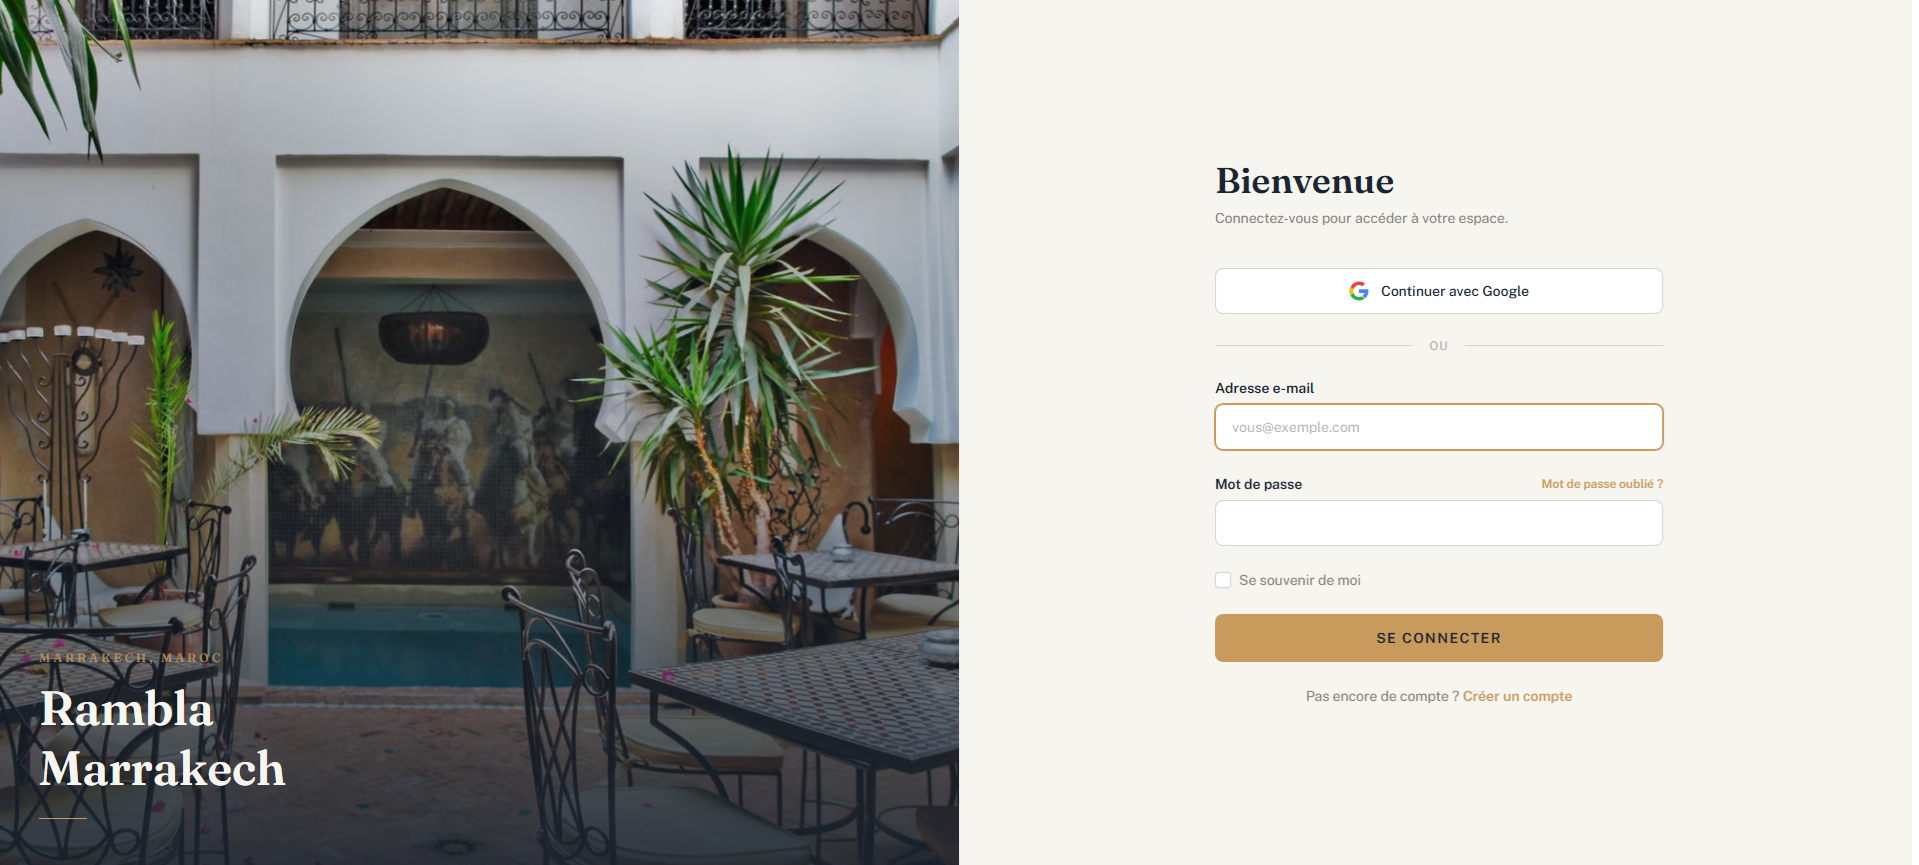
\includegraphics[width=0.90\textwidth,height=0.30\textheight,keepaspectratio]{screenshots/app-interface-login.png}
    \caption{Interface de connexion et d'authentification}
    \label{fig:interface-login}
\end{figure}

\begin{figure}[H]
    \centering
    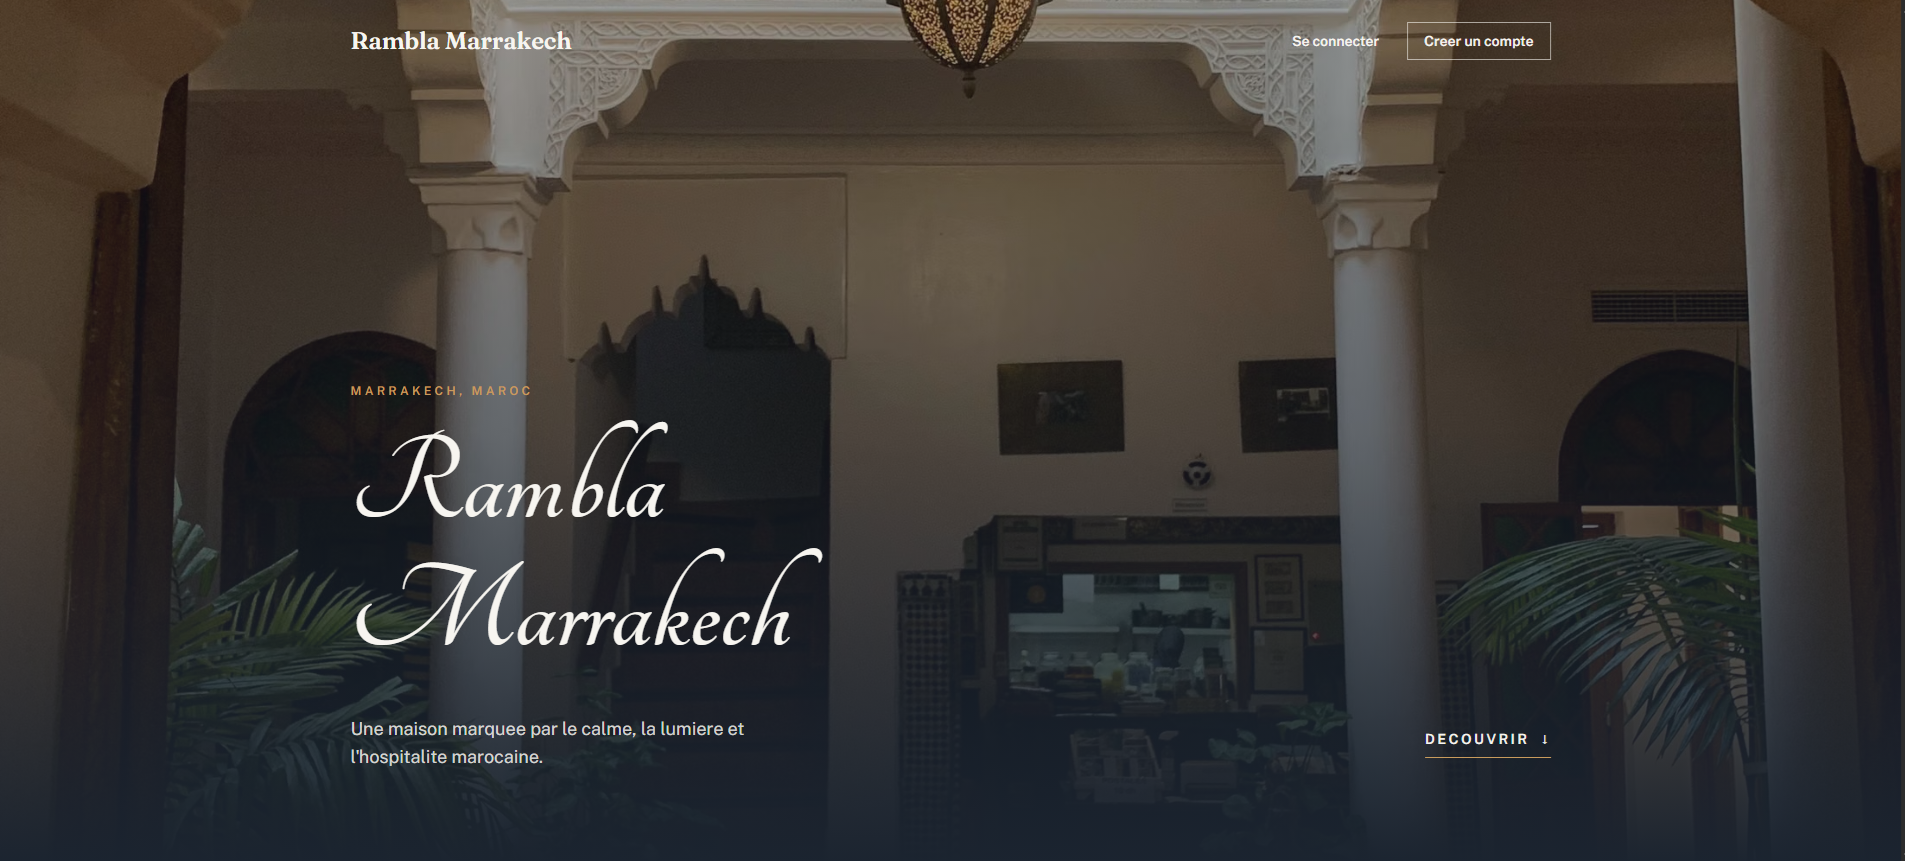
\includegraphics[width=0.90\textwidth,height=0.30\textheight,keepaspectratio]{screenshots/app-interface-home.png}
    \caption{Page d'accueil de la plateforme Rambla Marrakech}
    \label{fig:interface-home}
\end{figure}
\FloatBarrier

\Needspace{0.78\textheight}
\subsection{Page d'accueil et authentification}

La page d'accueil présente l'établissement et propose deux points d'entrée
principaux : la connexion et l'inscription. La page de connexion permet à
l'utilisateur de s'authentifier soit par un formulaire classique
(adresse électronique et mot de passe), soit par un bouton de connexion
via un compte Google, s'appuyant sur le protocole OAuth.

\Needspace{0.60\textheight}
\begin{figure}[H]
    \centering
    \includegraphics[width=0.90\textwidth,height=0.43\textheight,keepaspectratio]{screenshots/accueil.png}
    \caption{Page d'accueil et interface d'authentification}
    \label{fig:accueil}
\end{figure}
\FloatBarrier

\Needspace{0.78\textheight}
\subsection{Tableau de bord client}

Après connexion, le client accède à un tableau de bord synthétisant ses
commandes actives et ses réclamations en cours, ainsi que des accès
rapides vers les trois modules principaux : réservation, room service et
réclamations.

\begin{figure}[H]
    \centering
    \includegraphics[width=0.90\textwidth,height=0.43\textheight,keepaspectratio]{screenshots/dashboard-client.png}
    \caption{Tableau de bord de l'espace client}
    \label{fig:dashboard-client}
\end{figure}
\FloatBarrier

\Needspace{0.78\textheight}
\subsection{Formulaire de réservation}

Le formulaire de réservation présente une sélection du type de réservation
(chambre ou service) sous forme de cartes cliquables, un menu déroulant
listant les éléments disponibles avec leurs caractéristiques, ainsi qu'un
calendrier interactif permettant de choisir les dates d'arrivée et de
départ. Les dates déjà couvertes par une réservation existante apparaissent
grisées et non sélectionnables. Un message de disponibilité, actualisé en
temps réel, informe l'utilisateur avant même la soumission du formulaire.

\begin{figure}[H]
    \centering
    \includegraphics[width=0.90\textwidth,height=0.43\textheight,keepaspectratio]{screenshots/reservation-form.png}
    \caption{Formulaire de réservation avec calendrier interactif}
    \label{fig:reservation-form}
\end{figure}
\FloatBarrier

\Needspace{0.78\textheight}
\subsection{Espace Room Service}

Le module de room service présente le menu du restaurant organisé par
catégorie sous forme de cartes illustrées. Chaque article dispose d'un
sélecteur de quantité et d'un bouton d'ajout à la commande. Une barre
récapitulative affiche le montant total ainsi qu'un bouton de validation
de la commande.

\begin{figure}[H]
    \centering
    \includegraphics[width=0.90\textwidth,height=0.43\textheight,keepaspectratio]{screenshots/room-service.png}
    \caption{Interface de commande room service}
    \label{fig:room-service}
\end{figure}
\FloatBarrier

\Needspace{0.78\textheight}
\subsection{Espace Serveur}

L'espace serveur présente la liste des commandes en cours sous forme de
cartes, chacune affichant la chambre concernée, le détail des articles
commandés et le statut courant. Un bouton d'action permet de faire
progresser la commande vers l'étape suivante du cycle de préparation.

\begin{figure}[H]
    \centering
    \includegraphics[width=0.90\textwidth,height=0.43\textheight,keepaspectratio]{screenshots/staff-orders.png}
    \caption{Interface de suivi des commandes côté serveur}
    \label{fig:staff-orders}
\end{figure}
\FloatBarrier

\Needspace{0.78\textheight}
\subsection{Espace Administration}

Le tableau de bord de l'administration met en évidence le nombre de
réclamations urgentes non résolues. La liste des réclamations présente
chaque incident avec un indicateur visuel de priorité et des boutons
d'assignation et de résolution. La liste des réservations en attente
propose des boutons de confirmation et d'annulation, comme illustré par les
Figures~\ref{fig:admin-complaints} et~\ref{fig:admin-reservations}.

\begin{figure}[H]
    \centering
    \includegraphics[width=0.90\textwidth,height=0.43\textheight,keepaspectratio]{screenshots/admin-complaints.png}
    \caption{Interface de gestion des réclamations côté administration}
    \label{fig:admin-complaints}
\end{figure}
\FloatBarrier

\begin{figure}[H]
    \centering
    \includegraphics[width=0.90\textwidth,height=0.43\textheight,keepaspectratio]{screenshots/admin-reservations.png}
    \caption{Interface de gestion des réservations côté administration}
    \label{fig:admin-reservations}
\end{figure}
\FloatBarrier

\section{Conclusion}

Ce chapitre a présenté la structure générale du projet ainsi que les
principales interfaces de la plateforme, en mettant en évidence les objets
interactifs proposés à chaque type d'utilisateur. Ces éléments illustrent
concrètement la mise en œuvre des mécanismes conçus au chapitre précédent.


% ─────────────────────────────────────────────────────────────────────────
% CONCLUSION GÉNÉRALE
% ─────────────────────────────────────────────────────────────────────────
\chapter*{Conclusion générale et perspectives}
\addcontentsline{toc}{chapter}{Conclusion générale et perspectives}

Ce projet de fin d'année a permis de concevoir et de mettre en œuvre une
plateforme web répondant aux besoins de dématérialisation des services
d'un établissement hôtelier, conduite selon la méthode agile Scrum en
cinq sprints. Une plateforme structurée autour de trois espaces
utilisateurs a été développée, couvrant la réservation de chambres et de
services, la gestion du room service et le traitement priorisé des
réclamations techniques.

Les tests réalisés ont permis de valider le bon fonctionnement de
l'ensemble des modules ainsi que la fiabilité du contrôle d'accès par
rôle et de la prévention des conflits de réservation. Les perspectives
dégagées, notamment l'intégration d'une communication en temps réel et le
développement d'une application mobile, ouvrent des pistes concrètes pour
la poursuite de ce travail.

% ─────────────────────────────────────────────────────────────────────────
% RÉFÉRENCES
% ─────────────────────────────────────────────────────────────────────────
\begin{thebibliography}{99}
    \addcontentsline{toc}{chapter}{Références}

    \bibitem{laravel} Laravel Documentation. Disponible à l'adresse :
    \url{https://laravel.com/docs} (consulté en 2026).

    \bibitem{tailwind} Tailwind CSS Documentation. Disponible à l'adresse :
    \url{https://tailwindcss.com/docs} (consulté en 2026).

\end{thebibliography}

% ─────────────────────────────────────────────────────────────────────────
% ANNEXES
% ─────────────────────────────────────────────────────────────────────────
\appendix
\chapter*{Annexes}
\addcontentsline{toc}{chapter}{Annexes}

\section*{Annexe A : Schéma de base de données}

Le schéma de base de données de la plateforme comprend les tables
suivantes : \texttt{users} (utilisateurs et rôles), \texttt{rooms}
(chambres), \texttt{room\_photos} (photographies des chambres),
\texttt{services} (prestations de l'hôtel), \texttt{reservations}
(réservations polymorphes chambre/service), \texttt{menu\_items} (articles
du restaurant), \texttt{orders} et \texttt{order\_items} (commandes de
room service), ainsi que \texttt{complaints} (réclamations techniques).

\section*{Annexe B : Extraits de code source}

Cette annexe présente deux extraits significatifs de la logique métier de
l'application, illustrant respectivement le mécanisme de contrôle d'accès
par rôle et la vérification de disponibilité des chambres.

\begin{lstlisting}[language=PHP, caption={Middleware de contrôle d'accès par rôle}, label={lst:checkrole}]
class CheckRole
{
    public function handle(Request $request, Closure $next, string ...$roles): Response
    {
        if (! in_array($request->user()?->role, $roles, true)) {
            abort(403);
        }

        return $next($request);
    }
}
\end{lstlisting}

Ce middleware illustre l'utilisation d'un nombre variable de paramètres
(\texttt{string ...\$roles}), permettant à une même route d'autoriser
plusieurs rôles simultanément (par exemple \texttt{role:technicien,admin}).

\begin{lstlisting}[language=PHP, caption={Vérification de disponibilité d'une chambre}, label={lst:isavailable}]
public function isAvailable($start, $end = null): bool
{
    $start = Carbon::parse($start);
    $end = $end ? Carbon::parse($end) : $start->copy()->addDay();

    $hasConflict = $this->reservations()
        ->whereIn('status', ['en_attente', 'confirmee'])
        ->where(function ($query) use ($start, $end) {
            $query->where(function ($q) use ($start, $end) {
                $q->whereNotNull('end_datetime')
                  ->where('start_datetime', '<', $end)
                  ->where('end_datetime', '>', $start);
            })->orWhere(function ($q) use ($start, $end) {
                $q->whereNull('end_datetime')
                  ->whereBetween('start_datetime', [$start, $end->copy()->subSecond()]);
            });
        })
        ->exists();

    return ! $hasConflict;
}
\end{lstlisting}

Cette méthode illustre la correction apportée à la logique de détection de
chevauchement décrite au Chapitre 4 : les deux cas de conflit (avec et
sans date de fin explicite) sont combinés au sein d'une unique requête,
avant l'application d'une seule négation sur le résultat global.

\end{document}
